\section{Reviewer-Auditable Boundary}

Reviewer-visible auditability complements row-level reproducibility with a release mode designed for sensitive speech evidence. Reviewers can inspect aggregate artifacts, figures, tables, manifests, validation gates, claim registries, agreement summaries, completion checks, and release-boundary statements. Raw transcript cases remain part of the governed local evidence layer.

\begin{figure}[htbp]
\centering
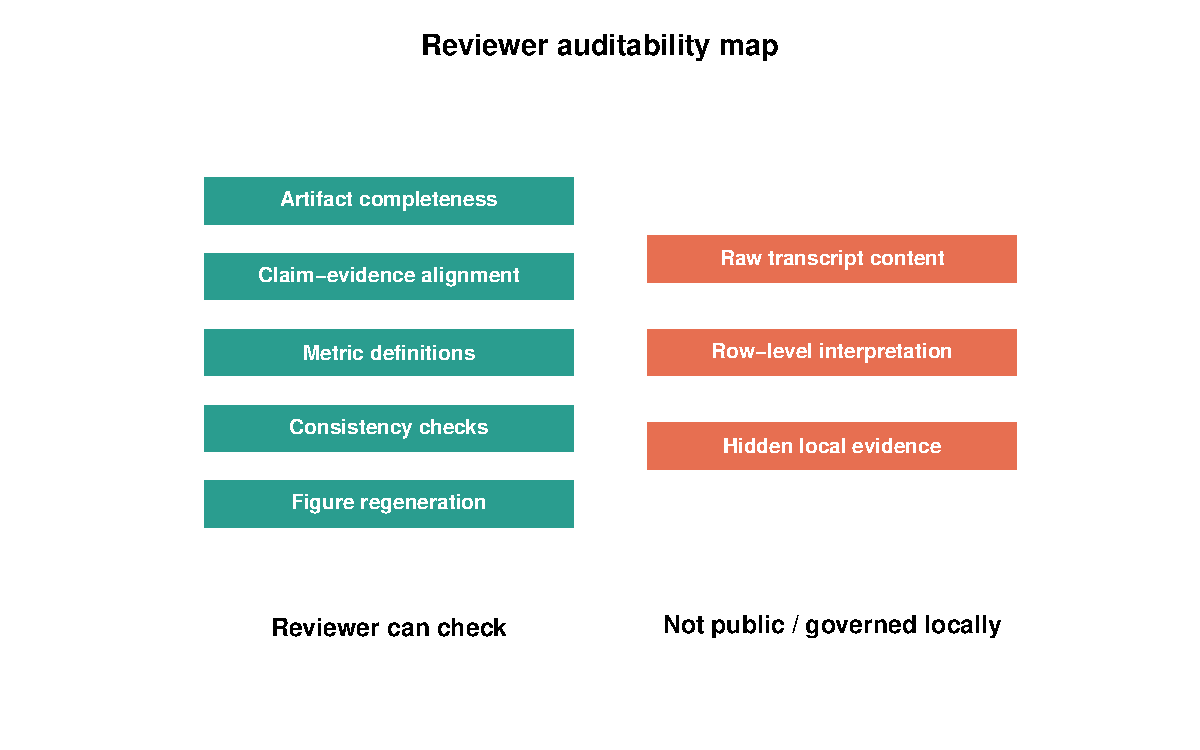
\includegraphics[width=.9\linewidth]{figures/fig4_artifact_audit_map.pdf}
\caption{Reviewer auditability map showing what can be checked and what remains local-only or institutionally governed. Generated by \artifact{build_fig4_artifact_audit_map.R}.}
\label{fig:audit_map}
\end{figure}

\begin{table}[htbp]
\centering
\caption{Reviewer audit checklist.}
\label{tab:reviewer_checklist}
\begin{tabularx}{\linewidth}{@{}LLL@{}}
\toprule
Reviewer check & Public evidence & Boundary \\
\midrule
Artifact completeness & Manifests and aggregate package list & Does not expose raw rows \\
Claim-evidence alignment & Claim registry & Claims remain scoped \\
Metric definitions & Method summary and metric audit & Raw transcripts not released \\
Consistency checks & Evidence-chain summaries & Aggregate validation only \\
Figure regeneration & R scripts and aggregate inputs & R scripts cannot access sensitive inputs \\
\bottomrule
\end{tabularx}
\end{table}

\begin{table}[htbp]
\centering
\caption{CDS-ASR case-study claim boundary table.}
\label{tab:case_boundaries}
\begin{tabularx}{\linewidth}{@{}LLL@{}}
\toprule
Case evidence & What it supports & Boundary \\
\midrule
258 ASR rows & Model-comparison context & Not deployment safety evidence \\
selected-300 provenance & Enriched audit surface & Not prevalence-preserving \\
30 reviewed rows & Human-reviewed audit layer & Single-expert audit \\
90 model assessments & Clustered metric evidence & Not independent calls \\
Aggregate replay & Policy-replay auditability & Retrospective, not live deployment \\
\bottomrule
\end{tabularx}
\end{table}

